\documentclass{article}

% math
\usepackage{amsmath}
\usepackage{amssymb}
\usepackage{siunitx}

% algorithms
\usepackage[algoruled,vlined]{algorithm2e}
\DontPrintSemicolon

% code
\usepackage{listings}

% lists
\usepackage{enumitem}

% font
\usepackage[tt=false]{libertine}
\usepackage{libertinust1math}
\usepackage[font={sf,small}]{caption} % caption font

% links and pdf index
\usepackage{hyperref}
\renewcommand{\subsectionautorefname}{section}

% bibliography
\usepackage[
    style=authoryear-comp,
    uniquename=false,
    uniquelist=false,
    date=year,
    backref=true,
]{biblatex}
\addbibresource{bibliography.bib}
\AtEveryBibitem{
    \iffieldundef{doi}{}{ % remove other links if there is a DOI
        \clearfield{url}
        \clearfield{eprint}
    }
    \iffieldundef{eprint}{}{ % remove url if there is an eprint
        \clearfield{url}
    }
    \clearfield{language} % guess what
    \clearfield{addendum} % remove my personal notes
}

% images
\usepackage{graphicx}
% command to center the contents even if they are larger than the text width
\newcommand{\widecenter}[1]{\noindent\hspace{-\textwidth}\makebox[3\textwidth][c]{#1}}
% command to include a pdf generated by matplotlib, 0.78125 = 360pt / 6.4in
\newcommand{\includempl}[1]{\includegraphics[scale=0.78125]{#1}}
\newcommand{\includemplhr}[1]{\includegraphics[scale=0.390625]{#1}}

% smaller margin notes
\let\oldmarginpar\marginpar
\renewcommand{\marginpar}[1]{\oldmarginpar{\sffamily\scriptsize #1}}
\setlength{\marginparwidth}{3.5cm}

% title
\title{Very fast Bayesian Additive Regression Trees on GPU}
\author{Giacomo Petrillo\\Department of Statistics, Computer Science,
Applications\\(DISIA), University of Florence\\
\href{mailto:giacomo.petrillo@unifi.it}{giacomo.petrillo@unifi.it}}

\begin{document}

    \maketitle

    \begin{abstract}
        
        Bayesian Additive Regression Trees (BART) is a nonparametric Bayesian regression technique. It is part of the toolbox of many statisticians. The overall statistical quality of the regression is typically higher than other generic alternatives, and it requires less manual tuning, making it a good default choice. However, it is a niche method compared to its natural competitor \texttt{XGBoost}, due to the longer running time, making sample sizes above \num{10000}--\num{100000} a nuisance. I present a GPU-enabled implementation of BART, faster by up to 200x relative to a single CPU core, making BART competitive in running time with \texttt{XGBoost}. This implementation is available in the Python package \texttt{bartz}.

    \end{abstract}

    \section{Introduction}
    \label{sec:intro}

    \paragraph{BART}

    Bayesian Additive Regression Trees (BART) is a nonparametric Bayesian regression method, introduced by \textcite{chipman2006,chipman2010}. It defines a prior distribution over the space of functions by representing them as a sum of binary decision trees, and then specifying a stochastic tree generation process. The posterior is then obtained with Metropolis-Gibbs sampling over the trees. See \textcite{hill2020} for a review, and \textcite[ch.~5]{daniels2023} for a textbook treatment.

    \paragraph{BART's success}
    
    BART has proven empirically effective, and is gaining popularity \autocite[consider, e.g.,][]{tan2019}. The Atlantic Causal Inference Conference (ACIC) Data Challenge has confirmed BART as one of the best regression methods for causal inference \autocite{dorie2019,hahn2019,acic2019,thal2023}. Many BART variants have been developed throughout the years, adding features such as variable selection \autocite{linero2018}.

    \paragraph{BART vs.\ XGBoost}

    According to the \textcite[p.~35]{kaggle2021} survey, the most popular regression method in the class of BART is the variant of gradient boosting implemented in the software \texttt{XGBoost} \autocite{chen2016}, used by half of the surveyed data scientists. \textcite[table~2, p.~1105]{linero2018b} show that BART predicts better than \texttt{XGBoost} on average on a set of benchmark datasets (with both methods cross validated). The other advantages of BART over \texttt{XGBoost} are that, due to being Bayesian, it provides full uncertainty quantification out of the box, a principled way to extend the model for special settings, and good results even without cross validation. However, BART is much slower than \texttt{XGBoost}, making it impractical for large datasets: the largest BART analysis I have encountered had $n\approx\num{500000}$ observations/examples and $p=90$ predictors/features \autocite{pratola2020}, while \texttt{XGBoost} boasts ``billions of examples'' on its home page.

    \paragraph{XBART}

    \textcite{he2019,he2021} introduced Accelerated BART (XBART), a BART variant that partially sacrifices Bayesianism to run 20--30 times faster. They show XBART is overall better at prediction than Random Forests and \texttt{XGBoost}, by working well in both high and low noise settings. However, to this day, XBART seems to not have gained traction. I believe this is due to the lack of a welcoming software ecosystem and publicity, rather than a problem with the method. XBART, not being fully Bayesian, also loses the advantage of a well-defined way of extending the model, which is important in Statistics.

    \paragraph{BART on GPU}

    To tackle this challenge, and bring the features of BART to large datasets, I re-implemented the original BART algorithm for GPU. My implementation yields a speed gain of up to 200 times, comparing a Nvidia A100 GPU against a single Apple M1 Pro CPU core. The maximum gain can be reached only with sample size $n \gtrsim \num{1000000}$ and  number of predictors and number of trees $p,n_\text{tree}\lesssim 1000$, but these limits look solvable with additional work. I provide a Python package, \texttt{bartz} \autocite{petrillo2024b}, which mimics the most common BART interface found in R packages.

    \section{BART recap}

    \paragraph{Bayesian nonparametric regression}

    BART is a Bayesian nonparametric regression method, i.e., given a set of $n$ pairs of observations $(\mathbf x_i,y_i) \in \mathbb R^p \times \mathbb R$, it infers without guidance a function $f$ such that $y_i = f(\mathbf x_i) + \varepsilon_i$, keeping a balance between $f$ and the error terms $\varepsilon_i$ such that given a new $\mathbf x^*$ from a pair $(\mathbf x^*, y^*)$ with $y^*$ yet unknown, $f(\mathbf x^*)$ is a good advance prediction of $y^*$. The result is provided in the form of a set of possible functions $\{f_k\}$, chosen in such a way that the spread of $f_k(\mathbf x^*)$ over the possibilities quantifies the uncertainty in predicting $y^*$. See \textcite[ch.~4]{muller2015}.

    \paragraph{BART in brief}

    BART represents the regression function as the sum of many decision trees. It puts a prior probability distribution over the space of all possible trees, and then samples from the distribution conditioned on the observed datapoints with a MCMC. This provides a posterior distribution over the space of trees, in the form of a set of random samples from such distribution, which represent the inference about which functions could describe the data. The pointwise average of these samples gives a single pointwise good estimate, while the pointwise standard deviation a pointwise uncertainty quantification.

    \paragraph{Implementations}

    The most popular implementations of BART are the R software libraries \texttt{bartMachine} \autocite{kapelner2016,kapelner2023}, \texttt{dbarts} \autocite{dorie2024}, and \texttt{BART} \autocite{sparapani2021,mcculloch2024}, though many others exist.

    \subsection{Definition of the BART model and prior distribution}
    \label{sec:bartprior}

    I summarize the description from the original BART paper \autocite{chipman2010}.

    \paragraph{Decision trees}
    
    A decision tree is a way to represent a stepwise function $\mathbb R^p \to \mathbb R$ using a binary tree. Each non-leaf node contains a splitting axis $i$ and a splitting point $s$, partitioning the input space in two half-spaces along the plane $\{\mathbf x \in \mathbb R^p: x_i = s\}$, orthogonal to axis $i$. Each half is assigned to a children. Children nodes in turn further divide their space amongst their own children. Leaf nodes contain the constant function value to be associated to their whole assigned rectangular subregion. A minimal tree consisting of a single root leaf node represents a flat function. See \autoref{fig:tree} for an illustration.

    \begin{figure}
        \widecenter{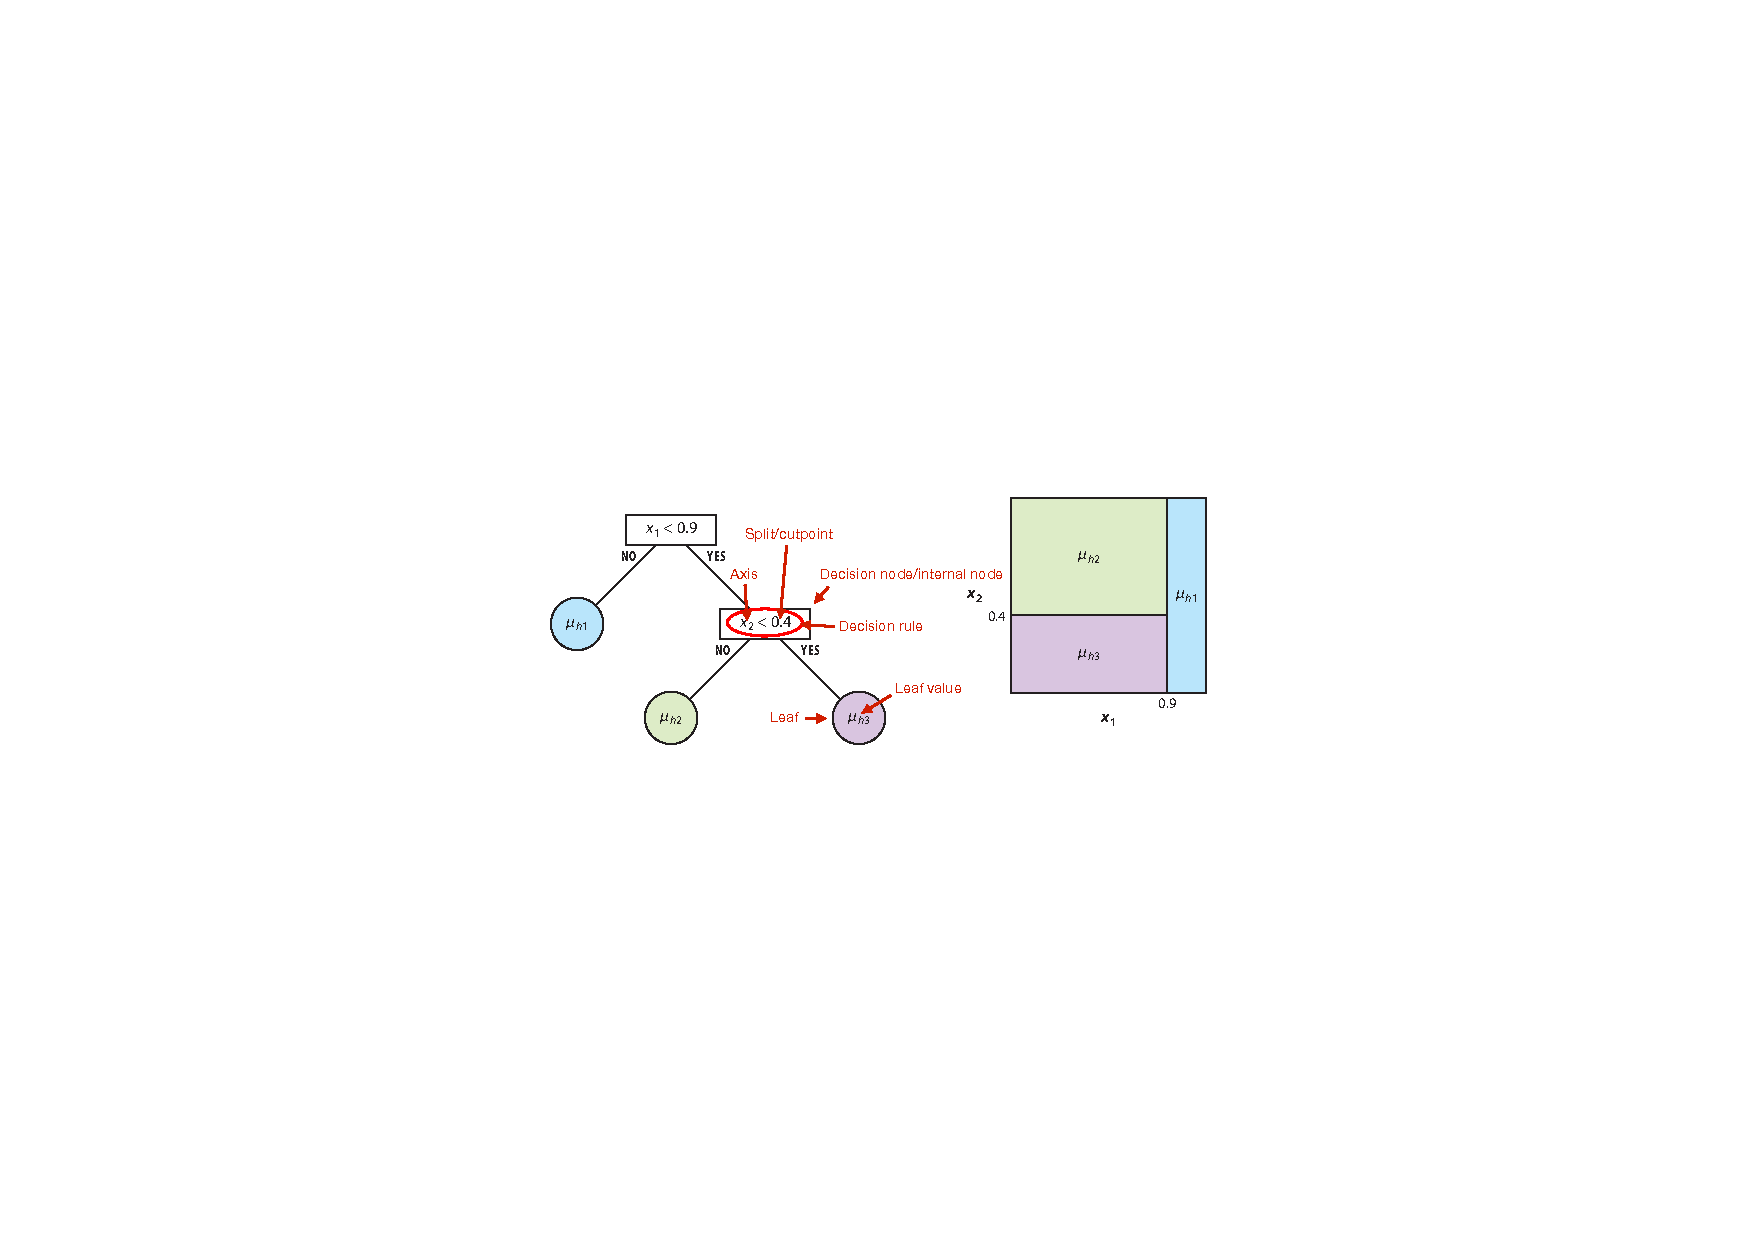
\includegraphics[width=\textwidth]{fig1hill2020.pdf}}
        \caption{\label{fig:tree} Depiction and terminology of a decision tree. Adapted from \textcite{hill2020}.}
    \end{figure}

    \paragraph{Decision trees for regression}
    
    A decision tree can be used to represent a parametrized family of functions for regression. The parameters are the structure of the tree $T$, including splitting decisions, and the leaf values $M$. I indicate the function represented by the tree with $g(\mathbf x;T,M)$. To use this model in Bayesian inference, it is necessary to specify a prior distribution over $(T,M)$. I factorize the prior as $p(T,M) = p(M\mid T) p(T)$ and specify the two parts separately.

    \paragraph{Prior over tree structure}
    
    The distribution $p(T)$ is defined by the following recursive generative model \autocite[see][]{chipman1998}. Fix an axes-aligned grid in the input space, not necessarily evenly spaced, by specifying a set of splitting points $S_i = \{s_{i1}, \ldots, s_{in_i}\}$ for each axis $i \in \{1,\ldots,p\}$. Start generating the tree from the root, descending as nodes are added. At each new node, consider the subset of splitting points which are available in its assigned subregion along each axis, and keep only the axes with at least one split available. If there are none, the node is a leaf. If there are any, decide with probability $P_d = \alpha/(1 + d)^\beta$ if the node is nonterminal, i.e., if it should have children, where $d$ is the depth of the node, $d=0$ at the root, and $\alpha \in [0, 1]$ and $\beta \in [0,\infty)$ are two fixed hyperparameters. If the node is nonterminal, its splitting axis is drawn uniformly at random from the allowed ones, and the splitting point along the chosen axis is drawn uniformly at random from the available ones.

    \paragraph{Prior over leaf values}
    
    If a node terminates, its leaf function value is sampled from a Normal distribution with mean $\mu_\mu$ and standard deviation $\sigma_\mu$, independently of other leaves. This defines $p(M\mid T)$.

    \paragraph{Complete regression model}
    
    The BART regression model uses a sum of $m$ independent trees, each with the prior above:
    %
    \begin{align}
        %
        y_i &= f(\mathbf x_i) + \varepsilon_i, &
        %
        \varepsilon_i \mid\sigma &\overset{i.i.d.}\sim \mathcal \mathcal N(0, \sigma^2), &
        %
        &p(\{T_j\}, \{M_j\}) = \notag \\
        %
        f(\mathbf x) &= \sum_{j=1}^m g(\mathbf x; T_j, M_j), &
        %
        \frac{\lambda\nu}{\sigma^2} &\sim \chi^2_\nu, &
        %
        &\quad = \prod_{j=1}^m p(M_j \mid T_j) p(T_j). \label{eq:bartdef}
        %
    \end{align}

    \paragraph{Hyperparameters}
    
    The free hyperparameters in the model, to be chosen by the user, are:
    %
    \begin{itemize}

        \item The splitting grid. The two common defaults are 100 equally spaced splits along each $\mathbf x$ axis in the range of the data, or a split midway between each observed value along each $\mathbf x$ axis.
        
        \item The number of trees $m$, default 200. This should grow with the sample size, but there is no known precise scaling.
        
        \item $\alpha$ and $\beta$, regulating the depth distribution of the
        trees. Default 0.95 and 2.
        
        \item $\mu_\mu$ and $\sigma_\mu$, which set the prior mean and variance
        $m\mu_\mu$ and $m\sigma_\mu^2$ of $f(\mathbf x)$. By default set based on some measure of the location and scale of the data.
        
        \item $\nu$ and $\lambda$, which regulate the prior on the variance of the error term. By default $\nu=3$, while $\lambda$ is set to some measure of squared scale of the data.

    \end{itemize}

    \subsection{BART inference procedure and posterior distribution}

    I first succintly recap applied Bayesian inference, then proceed with the specific procedure used in BART. See \textcites{chipman1998,chipman2010}[\S A]{kapelner2016}[ch.~5]{daniels2023}[\S2.1.4, p.~5]{tan2019} for further details.

    \paragraph{Bayesian inference}

    In the Bayesian paradigm, the parameters of the model (and consequently the predictions) are inferred from the data by conditioning the prior probability distribution on the observed values of the data, obtaining a posterior distribution for the parameters. The model definition in \autoref{eq:bartdef} can be expanded into a joint probability density function of the data and parameters $p(\mathbf y, \sigma, \{T_j\}, \{M_j\})$, and the posterior $p(\sigma, \{T_j\}, \{M_j\}\mid \mathbf y)$ is, up to a constant factor, the same expression but with $\mathbf y$ held fixed at the observed values. This distribution expresses the degree of belief in each possible combination of parameter values being the correct one; e.g., the mode or the mean of the distribution are good estimates of the parameters.

    \paragraph{MCMC}

    Even though the posterior $p(\sigma, \{T_j\}, \{M_j\}\mid \mathbf y)$ could be written down explicitly, it is a long and complex formula that is in practice impossible to interpret. To represent the posterior in a legible way, the most common technique is Markov chain Monte Carlo (MCMC): it is possible to define an iterative numerical procedure that, starting from an initial choice of parameter values, evaluating numerically the posterior only in some points, picks a new set of values, and so on, yielding overall a sequence of parameter values which is a random sample from the posterior. Then, e.g., the mean of the distribution is approximated by the average of these samples. See \textcite{brooks2011} for a reference on MCMC.

    \paragraph{Properties of MCMC}

    The samples produced by MCMC are only asymptotically correct: the chain takes some time to ``forget'' the arbitrary initial state and start sampling from the actual distribution. They are also not independent, as each sample is picked starting from the previous one. In practice, some of the initial samples must be discarded, and the total number of samples must be higher than what's needed.

    \paragraph{Metropolis sampler}

    A common general way of building a MCMC is the Metropolis-Hastings class of samplers. A MH sampler requires to define a ``proposal distribution''. The proposal is parametrized by the current values of the parameters in the chain. A random draw from the proposal gives potential new parameter values. Then a criterion decides if the new proposed values are accepted (keep new values) or rejected (keep current values), with a biased coin flip that depends on the posterior. In other words, the sampler tries to move one step at a time in parameter space, picking a move at random, testing the ground, and deciding whether to proceed in that direction, based on how much the probability increases going there.

    \paragraph{Gibbs sampler}

    Another general way of defining a MCMC is Gibbs sampling, based on partioning the procedure across parameters. If there are many parameters, it is difficult to devise a good proposal distribution for Metropolis, or to find other valid schemes in general. It is possible to sample only one parameter (or one subset of parameters) at a time, while keeping the other parameters fixed to their current values, as if those other values were known in advance. Iterating this over all parameters produces a valid MCMC.

    \paragraph{The BART MCMC}

    BART uses Metropolis sampling and exact sampling within a Gibbs sampler. The partition for Gibbs is: the structure of each tree $T_j$, the leaves of each tree $M_j$, and the error variance $\sigma$. Each $T_j$ is sampled with Metropolis, while each $M_j$ and $\sigma$ are sampled exactly because their conditional posteriors are standard distributions. More in detail, each iteration of the MCMC proceeds as follows. A random small modification is proposed for $T_1$, proposing to grow a leaf into a node with two leaves, to prune two sibling leaves making their parent a leaf, or other more complex moves. It is either accepted or rejected. Then, $M_1$ is sampled given the potentially modified $T_1$; this step is a linear regression. This is repeated for all trees in order. Then $\sigma$ is sampled with the trees fixed; its conditional posterior is an inverse gamma distribution.

    \paragraph{Behavior of the BART MCMC}

    The following is based on my general experience with BART and with developing the implementation described in this paper. The acceptance of the tree structure Metropolis step is typically \SI{10}\%--\SI{30}\% \autocite[see also][891]{pratola2016}, so on average the whole forest moves every 3 to 10 MCMC iterations. Pathological cases can lower this acceptance to very small values. A rule of thumb on the number of samples is to run the chain for 2000 samples and discard the first 1000 (differently from the defaults of BART packages, which is discarding 200). It is useful to run at least 2 chains and compare the distributions of the function value at a few points; if the distributions do not coincide, it may be useful to burn more initial samples. Each tree should not end up with more than 10 leaves.

    \paragraph{Convergence of the BART MCMC}

    This MCMC is quite complex, and moves the tree structures slowly. In practice in most problems it will not reach convergence, i.e., it won't sample the tree structures from their actual posterior. However, the function values also depend on the leaves, which are re-sampled each time from scratch instead of updated with Metropolis, so the quality of the MCMC samples is sufficient for prediction, even if they are not representative of the precise tree distribution.

    \section{Implementation of BART on GPU}

    This is the principal contribution of this paper. The implementation described here corresponds to version 0.4.0 of the Python package \texttt{bartz} \autocite{petrillo2024b}.

    \paragraph{Tooling}

    I write the code in Python using the machine learning framework JAX \autocite{bradbury2018}. This is in contrast to almost all the existing implementations, that provide an R interface to lower-level code in C++ or Java. I believe the success of this implementation crucially depends on this choice of using modern ML tools instead of the ones typical of this field. JAX provides a computing toolset built around array objects, mimicking Numpy \autocite{harris2020}, and optimizes and compiles the sequence of operations for CPU, GPU or TPU.

    \subsection{Parallelism and branchlessness}

    \paragraph{Parallel computation}

    JAX automatically converts all the operations written in Python to GPU code. However, to actually gain from using the GPU, the operations must be easily parallelizable. For example: adding two large arrays elementwise is ok, because each sum can be executed independently; while a sequence of many different operations on a few values has to be executed sequentially. The GPU is slow at doing things in sequence, but can do many things at once.

    \paragraph{Branchless computation}

    Another property of the operations important for using JAX and the GPU effectively is the absence of branching. Branching means changing the sequence of planned operations based on a contextual condition; for example, an \texttt{if} clause that depends on the output of the previous calculation is branching, while an \texttt{if} clause that depends on a global configuration constant is not branching. In branchless code, the full sequence of arithmetic operations done by the code can be determined in advance, allowing to plan and optimize for optimal use of the GPU.

    \paragraph{Branchless \& parallel on CPU}

    Modern CPUs benefit as well, but to a lower degree, from branchless and parallelizable code. Branchlessness is important to make RAM access patterns predictable, which speeds up fetching data from memory (the slowest operation for the CPU), while parallelization happens at the levels of vectorized instructions and multiple cores.

    \paragraph{Branchless \& parallel BART}

    The BART MCMC algorithm does not look to have these properties: the sizes of the trees change as the algorithm runs, the size-changing modifications to the trees are accepted or rejected randomly, and each tree is processed after the previous one, so it is not possible to write it as a pre-determined sequence of arithmetic operations on large arrays. However, with a slight variation, this becomes possible. The variation is fixing a maximum depth for the trees. The BART prior is designed to favor shallow and balanced trees, and the well-functioning of the MCMC relies on the trees being shallow, so this is not a problematic restriction.

    \paragraph{Bottom line}

    To write an efficient JAX implementation of BART, I have to express the BART MCMC procedure as pre-determined arithmetic operations on large matrices.

    \subsection{Representation of variables}

    \paragraph{Trees}

    My goal is representing the trees in computer memory with a few large matrices of fixed size. The simplest way of doing this is with a heap, illustrated in \autoref{fig:heaptree}.
    %
    \begin{figure}
        \widecenter{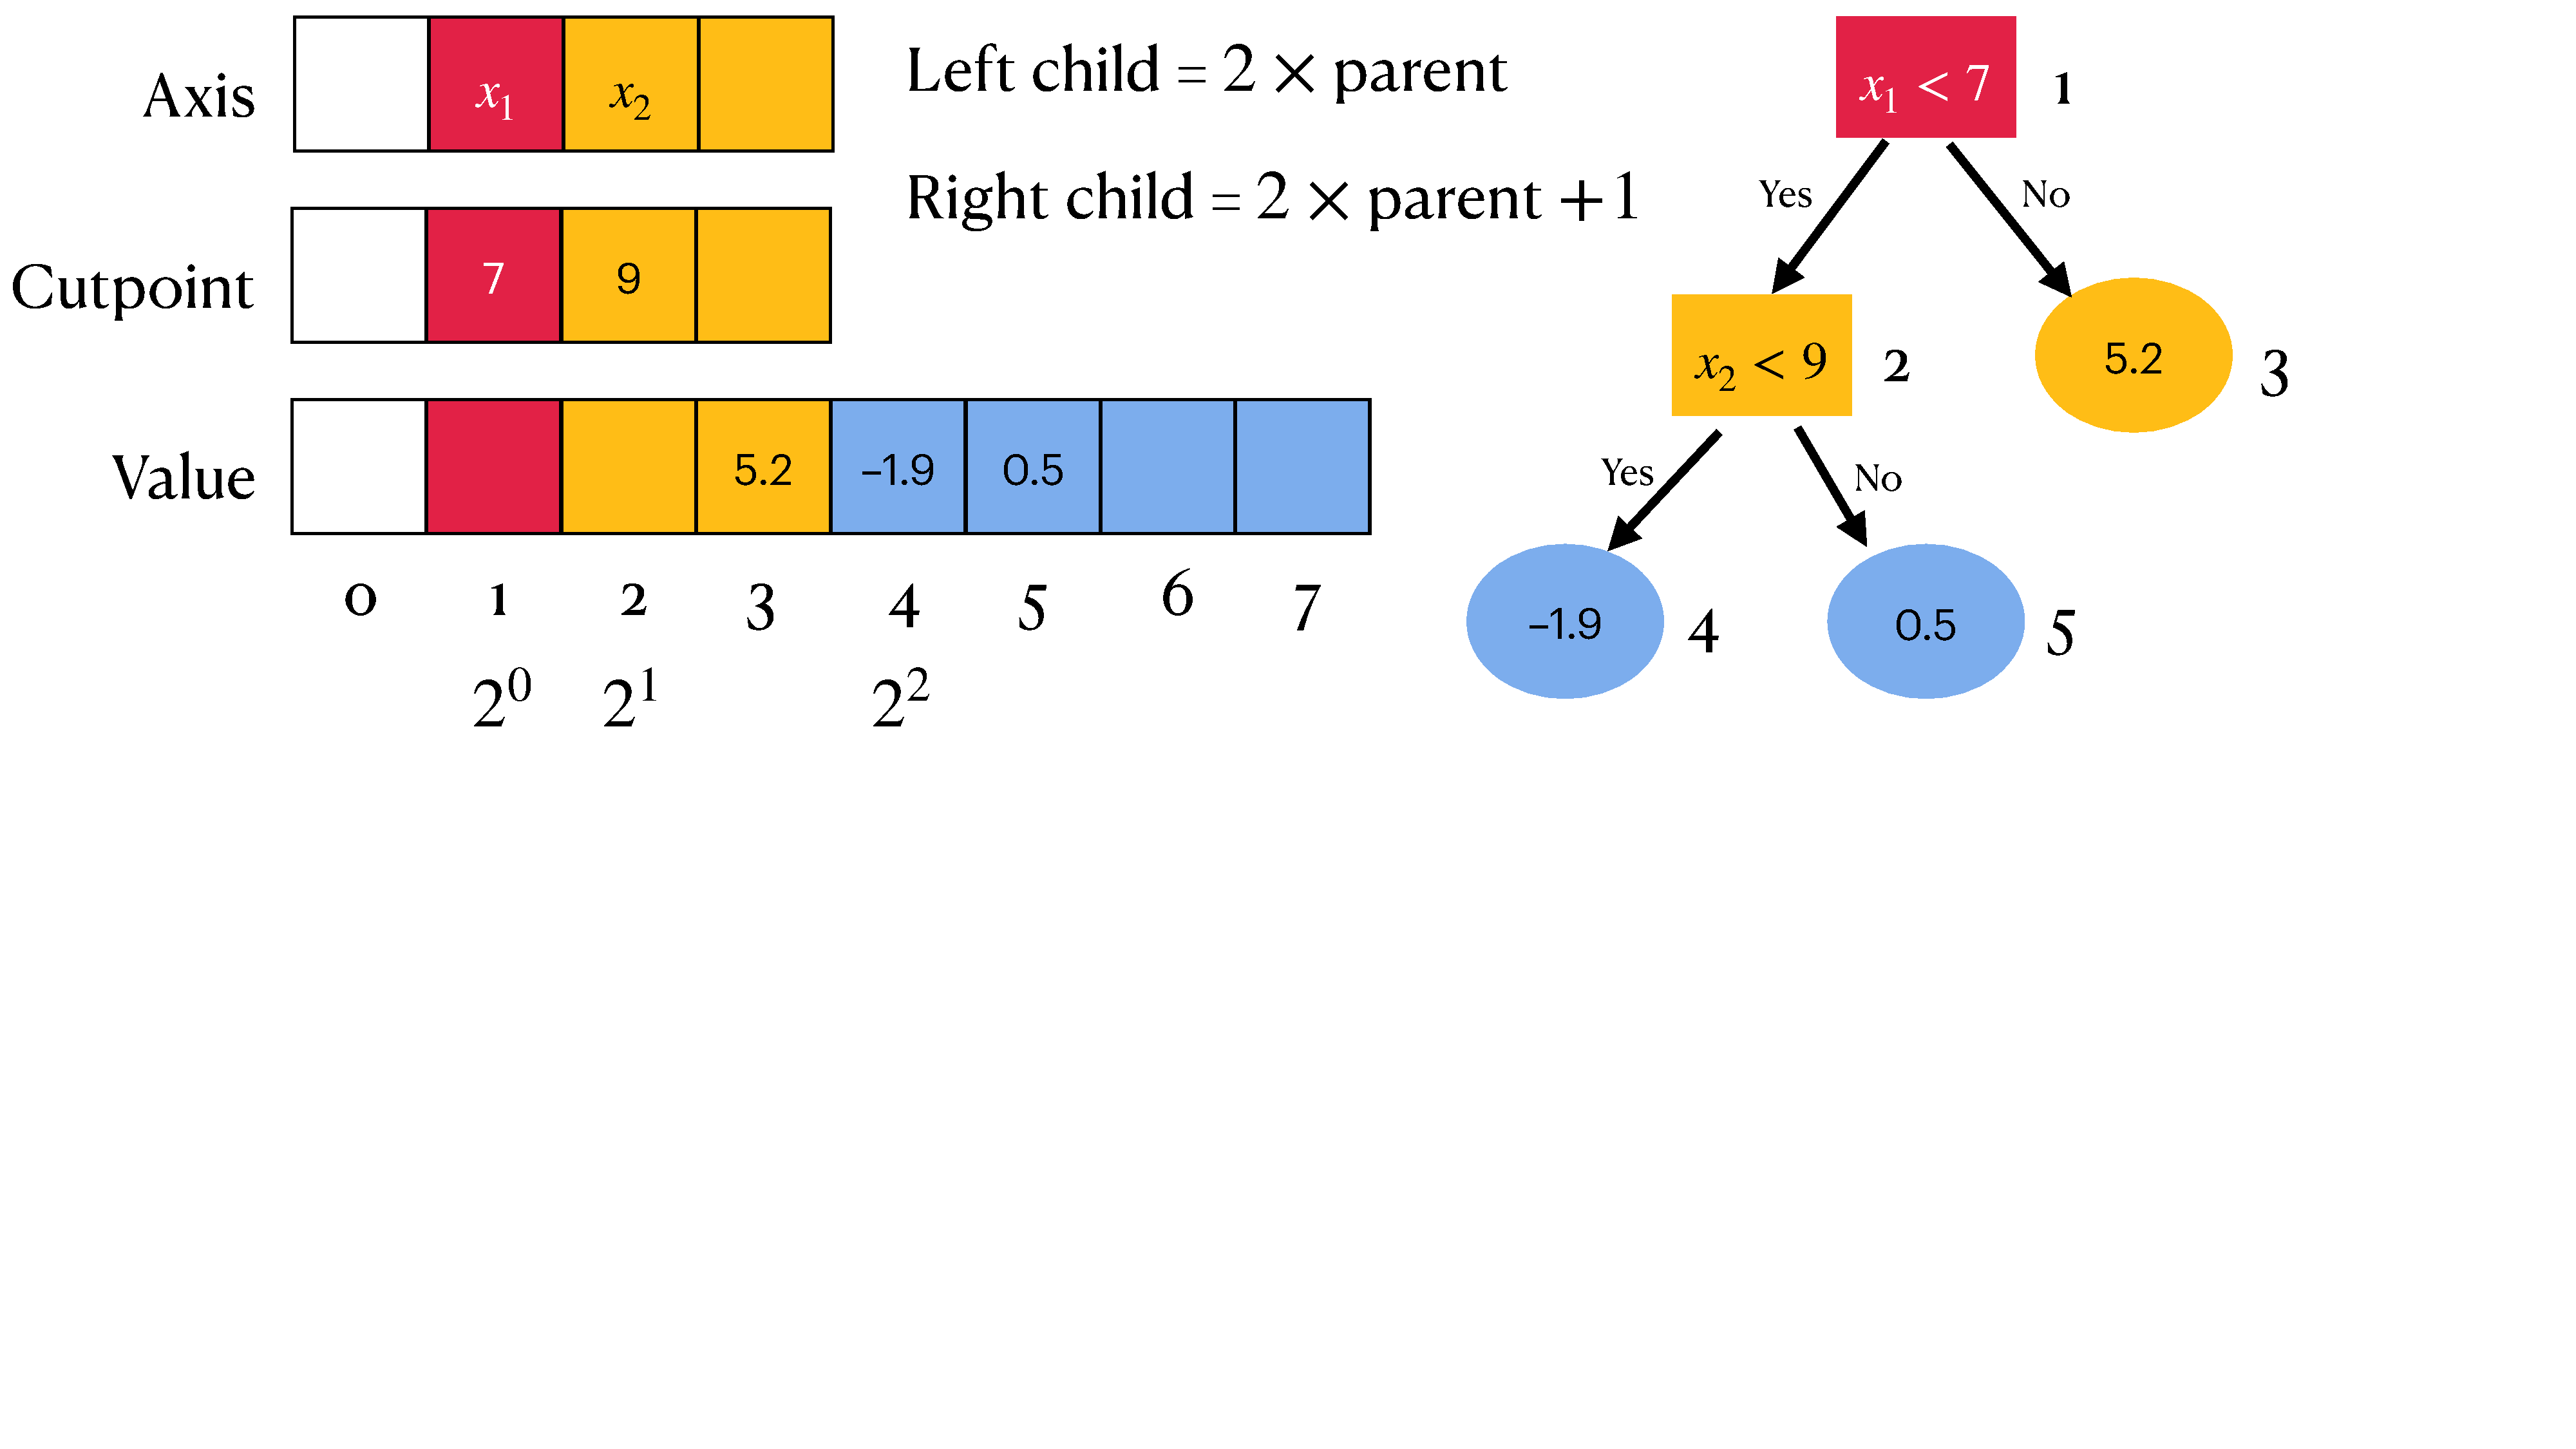
\includegraphics[width=\textwidth]{heaptree}}
        \caption{\label{fig:heaptree} Heap representation of a decision tree, with the maximum depth set to 3.}
    \end{figure}
    %
    Each tree is represented by 3 arrays, separately holding the axis and splitting point for decision nodes, and the value for leaf nodes. The arrays are fixed in size, and each index corresponds to a potential node in the tree. The indices are assigned in order, starting from 1, top to bottom, left to right (like reading text), imagining a full, balanced binary tree with the maximum allowed depth. The entries corresponding to nodes not actually present in the tree are ignored, as are respectively the axis and cutpoint entries/the value entry corresponding to leaf/decision nodes. I fix the convention that the cutpoints start from 1, and that a 0 value in the cutpoint array entry marks the node as a leaf. The set of trees is represented by 3 matrices where each row is a single tree array. I set as default, and always use in this article, maximum depth $D=6$, where $D=1$ for a root-only tree.

    \paragraph{Size of the tree representation}

    The heap representation of the trees wastes most of the array entries. However it turns out to use about the same memory as other common alternatives. The maximum number of nodes is $2^D - 1$, so the heap size is $2^D$ (index 0 is unused). Since the nodes at maximum depth can only be leaves, the axis and cutpoint arrays are only $2^{D-1}$ long. Using 32 bit integers and floats, the total size in bytes is $4 \times (2^{D-1} + 2^{D-1} + 2^{D}) = 2^{D+3}$ bytes. If $D=6$, that's 512 bytes. Consider instead a representation in C/C++ that used separately allocated linked node objects. Each node contains allocation metadata (16 bytes), axis (4), cutpoint (4), leaf value (4), and pointers to children ($2\times 8$), for a total of 44 bytes per node, rounded to 48 for alignment. This matches the size of the heap if there are 10 nodes per tree on average, and it's also not contiguous in memory. Other possible linked schemes, and those used in existing implementations, similarly consume a lot of memory in scaffolding; for example, \texttt{BART} uses 64 bytes per node. % see BART 2.9.6 files src/tree.h:100, src/tree.cpp:56

    \paragraph{Predictors}

    Each predictor $x_i$ can be replaced by its index into the splitting grid. Since the number of cutpoints never exceeds 255 in practice, each predictor then requires only 1 byte, for a total of $np$ bytes for the matrix of predictors. This size reduction is important because the whole matrix has to fit into the GPU memory, and it probably also speeds up fetching the predictors from memory as the algorithm runs.

    \subsection{The algorithm}

    I explain in full detail how to traverse the decision trees, as a simple illustration of how to write vectorized code, then describe the rest of the algorithm only in broad terms. See the software package documentation for details; the internals are documented.

    \paragraph{Traversing the trees}

    ``Traversing'' a decision tree means finding the leaf associated with a given $\mathbf x$ vector. This can be written as a loop through the levels of the tree, up to the maximum possible depth, carrying a flag to indicate whether the leaf has already been reached or not. This way the number of iterations of the loop is fixed in advance. See \autoref{alg:traverse}.
    %
    \begin{algorithm}[t]
        \KwData{Axis vector $\mathbf a$, cutpoint vector $\mathbf s$, predictors $\mathbf x$}
        \KwResult{Heap index of the leaf $\mathbf x$ falls into}
        leaf\_found = False\;
        index = 1\;
        \For(\hfill (the length of $\mathbf s$ and $\mathbf a$ is $2^{D-1}$\text{)}){i = 1 to $D - 1$}{
            axis = $a_\text{index}$\;
            split = $s_\text{index}$\;
            leaf\_found = leaf\_found OR (split = 0)\;
            child\_index = $2 \times \text{index} + (\text{1 \emph{if} $x_\text{axis} \ge \text{split}$ \emph{else} 0})$\;
            index = index \emph{if} leaf\_found \emph{else} child\_index\; 
        }
        \Return index
        \caption{\label{alg:traverse} Branchless traverse of a decision tree}
    \end{algorithm}
    %
    JAX automatically vectorizes the code: each operation in the traverse is repeated for all points and all trees. To repeat, it is not the whole algorithm which is run once for each combination of $\mathbf x$ and tree, but rather each operation in the algorithm is run on all combinations before moving to the next instruction, and the scalar variables become vectors or matrices as needed.

    \paragraph{Tree structure proposal}

    I have to propose a modification to each tree structure as moves for the Metropolis steps. The original BART picks at random amongst 4 types of moves: GROW (add two children to a leaf node), PRUNE (remove two sibling leaves), SWAP (permute the parameters of two directly related decision nodes), and CHANGE (change the parameters of a decision node) \autocite[\S5.1, p.~940]{chipman1998}. Following the implementation of \texttt{BART}, I use only GROW and PRUNE for simplicity \autocite[\S C, p.~57]{sparapani2021}. To stay branchless, I have to execute all the calculations for both moves, even if I end up using only one. GROW and PRUNE have the nice properties that the modifications can not overlap in the tree arrays, and that the tree proposed by GROW contains the initial tree which in turn contains the tree proposed by PRUNE. This allows to share the memory and most of the calculations between the two moves, and simplifies the operations with indices and residuals described next.

    \paragraph{Traverse indices cache}

    The indices that, for each tree, indicate in which leaf each datapoint falls into, are used to compute the acceptance probability of the Metropolis steps, and to sample the leaves. At each MCMC iteration, these indices change in limited ways due to the simplicity of the GROW and PRUNE moves, so it is convenient to keep the indices in memory rather than recompute them at each iteration. If the maximum depth of the trees $D$ is $\le 8$, the indices fit into a byte, so this cache uses $n \times n_\text{tree}$ bytes. Together with the $n\times p$ predictors matrix, this is the bulk of the memory usage of this algorithm.

    \paragraph{Residuals cache}

    A set of quantities used in all calculations are the residuals, i.e., the difference between the data $\mathbf y$ and the predictions of the tree ensemble. Computing the residuals is somewhat expensive, but they change progressively as each tree is modified in turn, so I keep a cache of residuals and, after sampling each tree, I add the difference between the old and new leaves. A potential problem is the accumulation of numerical error. The values of the residuals and their updates are similar across datapoints and trees, so, with 32 bit floats, each MCMC iteration adds a relative numerical error with standard deviation $\approx \num{1e-7} \sqrt m$. This is not a problem for all current BART applications, but it would be with 16 bit floats, which is an interesting option to further accelerate the implementation.

    \paragraph{Computations parallel across trees}

    The parts of the algorithm that can be parallelized across trees are:
    %
    \begin{enumerate}
        \item Propose the moves: since which move to use and the nodes to grow/prune are picked at random, there is no sequential dependence.
        
        \item Update the traverse indices cache based on the largest tree considered in each move: proposed for GROW, initial for PRUNE. The indices for the smaller version of the tree can be computed from these; this is done later on if the move is rejected/accepted.
        
        \item Count the number of points falling in each leaf. This is used to evaluate the acceptance probability and to sample the leaves. This only depends on the proposed moves.
        
        \item Compute the variance of the conditional posterior of each leaf. Since the calculation is a linear regression with Normal distributions, the variance only depends on the number of points and not on the values of the leaves, so there is no sequential dependence.
        
        \item Generate random samples. All random samples can be generated as standard uniform or Normal and transformed later to the target distribution. The leaves are  scaled immediately to their variance but left centered.
        
        \item Compute most of the terms in the Metropolis acceptance probabilities; similarly to the variances, many depend only on the number of points and fixed parameters.
    \end{enumerate}

    \paragraph{Computations sequential along trees}

    The parts that can't be parallelized are:
    %
    \begin{enumerate}[start=7]
        \item Sum the residuals falling in each leaf (bottleneck of the algorithm).

        \item For each leaf, add the initial leaf value times the number of points to the sum of residuals, to remove the effect of the current tree.

        \item Complete the calculation of the Metropolis acceptance probability and accept/reject the move.

        \item Compute the posterior mean of the leaves and add it to the pre-computed centered leaves.

        \item Add to the residuals the difference between the initial and new predictions of the tree.
    \end{enumerate}

    \paragraph{Bottleneck: summing residuals}

    The part that can not be parallelized across trees is problematic for the GPU. The main operation is summing the residuals. This kind of operation is called ``indexed reduce'': the residuals are summed in different accumulators (one per leaf), and which accumulator to use for each value is indicated by an array of indices (the traverse indices). This takes $O(n)$. Thus the GPU is fully utilized only if $n$ is high enough. As shown in \autoref{sec:perf} below, this is a problem in practice.

    \paragraph{Sampling the error variance}

    After the tree steps, the error variance is sampled using the sum of squared residuals to compute its conditional posterior. With many datapoints, the distribution is narrow, so this is approximately equivalent to setting the error variance to the variance not explained by the current trees.

    \subsection{Software package}

    I implemented the algorithm in the Python package \texttt{bartz}, distributed through PyPI \autocite{petrillo2024b}. The code is available under the permissive MIT open-source license. The correctness of the implementation is checked with automatic unit tests. To ease adoption for new users, I provide an interface (in addition to lower-level functions) that imitates the popular and feature-rich package \texttt{BART}, which in turn shares most of the interface with \texttt{dbarts} and the historical implementation \texttt{BayesTree}. Some unit tests check that the samples produced by \texttt{bartz} and \texttt{BART} with the same configuration represent the same posterior. The prototype usage is
    %
    \lstset{
        language=Python,
        basicstyle=\ttfamily\small,
        commentstyle=\itshape,
    }
\begin{lstlisting}
import bartz
X, y, X_test = ... # fetch data
bart = bartz.BART.gbart(X, y, ...) # run the MCMC
y_pred = bart.predict(X_test) # predict at new locations
\end{lstlisting}

    \section{Performance measurements}
    \label{sec:perf}

    In \autoref{sec:speed} I measure the running speed of the algorithm, while in \autoref{sec:pred} I check its correctness.

    \subsection{Speed benchmark}
    \label{sec:speed}

    \paragraph{General setup}

    I pit my implementation \texttt{bartz} on CPU and GPU against \texttt{dbarts} (the fastest BART implementation) and \texttt{XGBoost}.\marginpar{Add XBART} My CPU is a single core of an Apple M1 Pro. As GPU, I use the Nvidia L4 for \texttt{XGBoost} and the Nvidia A100 for \texttt{bartz}. The L4 is smaller, but that does not make a difference for \texttt{XGBoost}, and it was more convenient to access. As performance metric I use the time per iteration; for BART, this is the time of a MCMC iteration, while for \texttt{XGBoost} this is the time to build all the trees, so they are not directly comparable. BART requires $O(1000)$ iterations for the MCMC, while \texttt{XGBoost} $O(100)$ for the cross validation, but can also be run just once with lower performance.

    \paragraph{Data generating process}

    I run the benchmark on synthetic data to set arbitrarily the dataset size $n$ and number of predictors $p$. For \texttt{bartz} I use a not particularly meaningful data generating process (DGP), designed purely for convenience in avoiding out-of-memory errors on large datasets:
    %
    \begin{align}
        y_i &= \cos\left( \frac{2n\pi}{32} \frac{i-1}{n-1} \right), \quad i = 1,\ldots, n, \\
        X_{ij} &= (i + (p+1)j) \bmod 256.
    \end{align}
    %
    Since \texttt{bartz} is branchless, the running time does not depend on the DGP, so the DGP does not need to be realistic. Instead, for \texttt{dbarts} and \texttt{XGBoost}, I have to specify a DGP that makes sense, otherwise their running time may vary substantially. I use
    %
    \begin{align}
        y_i &= \frac1{\sqrt p}\sum_{j=1}^p \cos(\pi X_{ij}) + \varepsilon_i, \\
        X_{ij} &\overset{\mathrm{i.i.d.}}{\sim} U(-2, 2), \\
        \varepsilon_i &\overset{\mathrm{i.i.d.}}{\sim} \mathcal N(0, 0.1^2).
    \end{align}
    %
    This is designed to be a realistic but ``easy'' DGP. The total data variance is $\approx 1$. $X$ is uniformly distributed, such that the evenly spaced splitting grid used by default in \texttt{dbarts} is optimal. The error standard deviation is 0.1, so the data is low noise enough for \texttt{XGBoost} to work well, but not so low noise that BART would have low acceptance problems in the MCMC. The model does not have interactions, so the algorithms should always find good decision rules.

    \paragraph{Size settings}

    The number of predictors and the number of trees influence the running time and the memory usage, so I repeat the benchmark on a $2\times 2$ grid of settings: low/high p $\times$ low/high number of trees. As ``low'' settings I use $p=100$, $n_\text{tree} = 200$, while as ``high'' I make the parameters grow proportionally to $n$ with $n/p = 10$ and $n/n_\text{tree}=8$. The number of trees being proportional to $n$ is an unusually high setting.\marginpar{This number of trees probably is too crazy high for XGBoost. I don't know how to set it sensibly. It shouldn't stay constant either.} These combinations are not optimal for inference, they are simple extreme cases to understand the computational complexity of the algorithms. The ``low-low'' setting is the one closer to common usage.

    \paragraph{Precise definition of iteration time}

    For BART, I am careful to measure only the time to run an iteration, after warming up, and not the time taken by initialization or post-processing. This is possible because both my package and \texttt{dbarts} allow to run each step of the algorithm separately. For \text{XGBoost}, instead, I measure the time to run it once with its default configuration; I expect this is indeed the time each fold in a CV would take and so it is the correct measure to make comparisons.\marginpar{I would really like an XGBoost expert to weigh in.}

    \paragraph{Results}

    The results are shown in \autoref{fig:time-all}. Consider the bottom-right panel, at ``low'' settings $p=100$, $n_\text{tree}=200$. \texttt{dbarts-cpu} is 3-4 times faster than \texttt{bartz-cpu} at low training set size $n$, then \texttt{bartz-cpu} catches up at $n\approx \num{20000}$ and they remain similar afterward. \texttt{bartz-A100} takes a constant time until $n \approx \num{1000000}$ where it starts following a linear trend, indicating full use of the GPU. At high $n$, \texttt{bartz-A100} is 200x faster than \texttt{bartz-cpu}, and 1000x faster than \texttt{xgboost-cpu}, making BART competitive with \texttt{XGBoost} after taking into account the different number of iterations required.

    \paragraph{Effect of limited GPU memory}

    A striking feature of \autoref{fig:time-all} is that with high $p$ or $n_\text{tree}$ the benchmark terminates at lower $n$. This is because I run out of GPU memory. The memory of GPUs is fixed, it can't be expanded, and there is no virtual memory, so this is an unavoidable limit. The speed premium of the GPU kicks in only at high $n$, so the memory limit indirectly limits the speed gain. The practical consequence is that running the algorithm in ``high'' $p$ or $n_\text{tree}$ settings allows a speed gain of at most 35x rather than the maximum 200x.

    \begin{figure}
        \widecenter{\includempl{time-all}}
        \caption{\label{fig:time-all} Time to run an iteration of the algorithm vs.\ sample size $n$, comparing \texttt{bartz} with the fastest BART implementation (\texttt{dbarts}) and \texttt{XGBoost}, for various settings of number of trees and number of predictors $p$. Keep into account that \texttt{XGBoost} requires only one iteration to produce a usable result, while BART requires $O(1000)$ iterations.}
    \end{figure}

    \paragraph{Memory usage}

    I was not able to reliably measure memory usage programmatically, but I observed on the system monitor that \texttt{bartz} uses $\approx n(p+n_\text{tree})$ bytes as expected, while \texttt{dbarts} uses $\approx 24 n(p+n_\text{tree})$. In my personal experience, memory usage is the showstopper in analysing large datasets.\marginpar{someone in the literature said the same, but I can't remember who} \texttt{dbarts} is the fastest package, but not the one with the lowest memory usage, as it caches the tree traverse like \texttt{bartz}, so this comparison does not necessarily make \texttt{bartz} state of the art re memory.

    \subsection{Predictive accuracy}
    \label{sec:pred}

    Since I re-implemented a well known algorithm, with unit tests checking that it yields the same results as an existing implementation, there is no need to measure its statistical performance thoroughly. However, to show at least one concrete piece of evidence that everything is working correctly, I run a comparison of the out-of-sample prediction error\marginpar{Measure also coverage.} between my package \texttt{bartz} and the 3 most popular BART implementations, on data simulated from a simple model with a dense linear term and a sparse quadratic term. The result is in \autoref{fig:rmse-all}; the RMSEs shake out similar within random variation as expected.

    \begin{figure}
        \widecenter{\includempl{rmse-all}}
        \caption{\label{fig:rmse-all} Test set root mean square error (RMSE) vs.\ training set size, comparing \texttt{bartz} with the most popular implementations of BART, to check they produce the same results, for various settings of number of trees and number of predictors $p$. The test set size is always 1000.}
    \end{figure}

    \paragraph{Data generating process}

    The data is simulated from the model
    %
    \begin{align}
        y_i &= \frac 1{\text{norm.}} \sum_{j=1}^p X_{ij} \beta_j + \frac 1{\text{norm.}} \sum_{j,k=1}^p A_{jk} X_{ij} X_{ik} + \varepsilon_i, \label{eq:rmsedgp} \\
        \varepsilon_i &\overset{\text{i.i.d.}}{\sim} \mathcal N(0, 1), \\
        X_{ij} &\overset{\text{i.i.d.}}{\sim} U(0, 1), \\
        \beta_j &\overset{\text{i.i.d.}}{\sim} \mathcal N(0, 1), \\
        A_{jk} &\begin{cases}
            \overset{\text{i.i.d.}}{\sim} \mathcal N(0, 1) & \text{if $\min(|j - k|, p - |j - k|) < 5$}, \\
            =0 & \text{otherwise},
        \end{cases}
    \end{align}
    %
    where the denominators ``norm.'' indicate standardization of the attached term to unit sample variance after generating the data, train and test set together. This step is improper, but the difference is small in high $n$, and the comparison is relative anyway. This standardization simplifies interpreting the RMSE, as the total variance of the data stays at about 3.

    \paragraph{On increasing the number of trees}

    Consider the top panels of \autoref{fig:rmse-all}. They both have the ``high'' $p$ setting, with $n = 10p$, while differring in the number of trees. In the right panel, at fixed $n_\text{tree}=200$, the RMSE at some point starts going up with $n$, while in the left panel it remains constant. This indicates that, at least with this kind of DGP, the number of trees should grow with $p$. Similarly, although much less markedly, comparing the bottom panels suggests that, as $n$ increases, at some point the number of trees should increase as well.

    At ``high'' $n_\text{tree}$, the series stop at $n\approx 8000$, which means $n_\text{tree}\approx 1000$. This is an unusually high setting. I've never seen more than 200 trees in the literature, but for \textcite[fig.~6, p.~286]{chipman2010} who reach $m=300$ as an experiment.

    The number of trees bears on the acceptance of the BART MCMC, together with the level of noise in the data. If the number of trees is too small, each tree has to grow deep to do its part in explaining the patterns in the data, and the MCMC gets stuck because ungrowing the trees is disfavored, and so they can't be changed in little steps; while with enough trees, each tree has to explain only a small part of the variation, so the prior prevails and keeps them shallow. The level of noise (i.e., unpredictable variation) has a similar effect: if the data is precisely predictable (for concreteness, picture $\operatorname{Std}[\mathbf y]/\sigma = 100$), the trees quickly grow to explain the variation, the error variance is shrunk accordingly, and once it is small, any small change that doesn't preserve a nigh-perfect data fit is too disfavored, so the MCMC gets stuck. Thus the signal/noise ratio (SNR) is an important influence on the optimal number of trees.\marginpar{Cite pratola?}

    I now make an informal argument about what the number of trees should be. The number of leaves in each tree is not fixed, but at equilibrium and with many trees there will be a typical value. As the leaf values determine the values of the function, the total number of leaves in the ensemble is the number of parameters of the regression. This number should be equal to the total number of degrees of freedom required to explain the function behind the data on the observed region. An upper bound on this is the number of observed points $n$. If the number of leaves per tree has to be $\lesssim 10$ for the well-functioning of the MCMC, then in the worst case there should be at least $n/10$ trees. The effective number of parameters depends on the properties of the function; for example, under this view, the increasing RMSE($n$) (with $p \propto n$) in the top-right panel of \autoref{fig:rmse-all} is due to the regression function (\autoref{eq:rmsedgp}) having a number of parameters $\propto p$.

    These considerations, together with the absence of high-$n_\text{tree}$ experiments in the literature, suggest this as an interesting area to explore, made accessible by this work as it alleviates the computational burden. I'll consider two specific examples. \textcite[\S4.1]{ronen2022} show numerically how the convergence of the MCMC degrades at high $n$. Their experiment is already computationally demanding, and they stick to the default 200 trees. A higher number of trees might improve the mixing. \textcite{pratola2016} develops complex Metropolis proposals to increase acceptance in high-$n$, low-$\sigma$ datasets; a simpler alternative solution might be again to increase the number of trees.

    \section{Conclusions}

    \paragraph{Main result}

    I devised a branchless version of the BART MCMC algorithm to run BART on GPU. This achieves a speedup sufficient to make BART competitive with \texttt{XGBoost}, the most popular tree-based method, making BART a concrete alternative with higher statistical quality. This speedup is possible only with $n\gtrsim\num{1000000}$, but this is the regime that matters anyway, as speed is less of a problem with less data.

    \paragraph{Mild limitations}

    Compared to \texttt{XGBoost}, the first evident limitation of my software package is that it does not implement regression with binary outcomes. The second one is that it runs on only one CPU core or GPU at once, while \texttt{XGBoost} allows to split data and processing across machines. This feature is straightforward to add, as JAX scales to large clusters, and the BART MCMC allows efficient sharding of the data \autocite{pratola2014}; I simply have not put in the work. In general my software is not mature and so does not provide a truly viable competitor to \texttt{XGBoost} right away.

    \paragraph{Deeper limitations}

    My implementation runs out of GPU memory when the number of predictors $p$ or the number of trees are high. This problem is unavoidable. The implementation already uses only 1 byte per predictor and 1 byte per tree index, so it's close to the minimum memory requirements. The indices cache could potentially be dropped, slowing down the algorithm, or batched from CPU memory; but the predictors matrix is always used all at once. It is possible to adapt the algorithm to run on multiple GPUs, but the partition has to be along the observations and not the predictors; if each GPU stores a small number of observations to fit a large number of predictors, there is no speed advantage.

    \paragraph{Future directions}

    Other than mundane improvements to the software, the most useful addition would be to re-implement XBART \autocite{he2021} for GPU as well. If XBART runs overall 20-30 times faster than BART, and \texttt{bartz} is 200x faster on GPU than the state of the art on CPU \texttt{dbarts}, hopefully XBART on GPU could be 4000x faster, making it decidedly advantageous compared to \texttt{XGBoost} or any other method. Since XBART uses an expensive single tree sampling process, scanning many predictors and splitting points to find good decision rules, it could potentially parallelize better at lower $n$, allowing to shard high-$p$ problems across GPUs without losing efficiency.

    \section*{Acknowledgements}

    I thank Antonio Linero, Andrew Herren, Richard P.\ Hahn, and Francesco C.\ Stingo for useful comments and suggestions. I did this work as a PhD candidate at the Department of Statistics, Computer Science, Applications (DISIA) ``G.~Parenti'' of the University of Florence (UNIFI), Italy, and as a visiting researcher at the Department of Statistics and Data Science (SDS) of the University of Texas at Austin (UT Austin), USA. The introductory material in sections~\ref{sec:intro} and~\ref{sec:bartprior} is adapted from \textcite{petrillo2024d} by the same author.

    \section*{Code and data}

    The results in this paper are fully reproducible with \textless ZENODO\textgreater.

    \printbibliography

\end{document}
